This chapter will present arguments for the validity of the results that can be
calculated with the implemented methods. At the same time the properties of
some setups are presented. All plots related to verification are generated in
the
python notebook \texttt{verifications.ipynb}.

\section{Scattering at a Single Interface}
In the most simple configuration, a single interface occurs at the boundary of
the two half spaces above and below the xy-plane.
The calculations for a transition from Copper to Silicon is shown in figure
\ref{fig:singleL} and figure \ref{fig:restsingle} in the appendix. In the case
of transversal horizontal polarisation, the analytical solution from equation
\ref{eq:theoSingleTH} yields the exact same results, as direct comparison of
the calculated values shows. For the other modes, no explicit analytical
solutions were found. However, the fulfilled sanity check for all results
gives a good argument for their validity.

Additionally, the behaviour of the transmittivity at the critical angles for
total reflection can be considered. Recalling that these mark the angles at
which a resulting mode changes to evanescent wave propagaion, we can calculate
critical angles for all possible transitions between incoming and outgoing
modes. These depend only on longitudinal and transversal velocities so that
the angles for all reasonable combinations are shown in table
\ref{tab:critangles}.
The critical angles for TH polarised waves are a subset of the critical angles
of the shown angles for L an TV polarised waves.

Comparing the obtained angles with the plots, we can see that these can explain
the kinks in the funtionality of reflectivity and transmittivity. For example,
in case of a longitudinal incident wave, the critical angle denotes the total
reflection at the transmitted TV mode. Despite this, the transmitted intensity
does not drop completely to zero as the transmitted longitudinal wave can still
transport energy.
\begin{table}[p]
    \centering
    \begin{tabular}{c||c|c|c|c}
                   & $c_{L,Cu}$  & $c_{T,Cu}$ & $c_{L,Si}$  & $c_{T,Si}$
        \\ \hline
        $c_{L,Cu}$ & \ang{90. }  & -          & \ang{34.42} & -
        \\
        $c_{T,Cu}$ & \ang{28.62} & \ang{90}   & \ang{15.71} & \ang{29.06}
    \end{tabular}
    \caption{Critical angles for transition from Copper to Silicon depending on
        velocity of the incoming mode (rows) and outgoing mode (columns)}
    \label{tab:critangles}
\end{table}

\begin{figure}[p]
    \centering
    \begin{subfigure}{0.8\textwidth}
        \includegraphics[width=\textwidth]{/singleinterface/TH_CuSi}
        \caption{Scattering of TH polarised waves at a single interface}
        \label{fig:singleL}
    \end{subfigure}\\ \vspace{0.75cm}
    \begin{subfigure}{0.8\textwidth}
        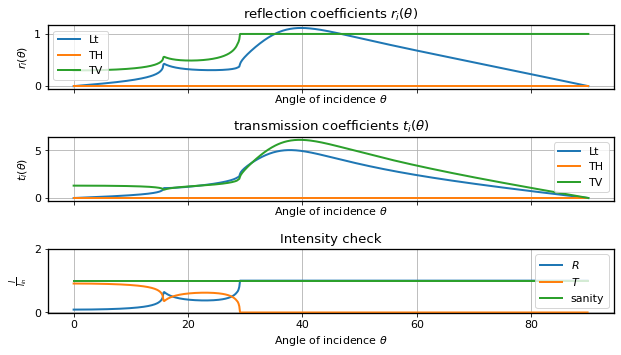
\includegraphics[width=\textwidth]{/singleinterface/TV_CuSi}
        \caption{Scattering of TV polarised waves at a single interface}
    \end{subfigure}
    \caption{}
    \label{fig:restsingle}
\end{figure}

\begin{figure}[h]
    \centering
    \includegraphics[width=\textwidth]{../pictures/singleinterface/TH_CuSi}
    \caption{Scattering of L polarised waves at a single interface}
    \label{fig:singleL}
\end{figure}

\section{Multilayer Structures} \label{sec:reflector}
Here an example multilayer structure is presented. According to
\cite{Satoh2005} multilayer structures consisting of low impedance
$\si{SiO_2}$ and high impedance metals like tungsten or molybdenum are
suitable for fabrication of acoustic resonators. For that reason the following
plots present simulation result of bragg reflector with a unit cell of
$\si{SiO_2}$ and Mo which is repeated eight times and with an embedding layer
of $\si{SiO_2}$. The thicknesses are chosen to be a quarter wavelength of 
a wave with frequency $f_0=100\si{GHz}$  with
 longitudinal polarisation. With longitudinal velocity
$c_{L,SiO2}=8478\si{\frac{m}{s}}$
and transversal velocity $c_{T,SiO2} = 4725\si{\frac{m}{s}}$ of $\si{SiO_2}$ and
velocities $c_{L,W} = 5160\si{\frac{m}{s}}$ and $ c_{T,W} = 2843\si{\frac{m}{s}}$ 
of tungsten  these thicknesses are
$d_1=13.98\si{nm}$ for $\si{SiO_2}$ and $d_2 = 19.16\si{nm}$ for tungsten.
The overview plots for calculations with all angles are shown in figures
\ref{fig:totalMultiL} to \ref{fig:totalMultiTV} for each mode. The positions
of the bandgap at $f_0$ is clearly visible in the longitudinal case and it 
appears that only uneven orders from equation \ref{eq:posBandgap} are visible
under normal incidence, because of the construction with layers of 
quarter wavelength thickness. This changes for larger angles where the phase shift 
per layer becomes dependent on the incident angle and mode.
In \ttt{verifications.ipynb}, also the case of normal incidence can be examined
and the positions of the bandgaps can be compared to the theoretical expectations
from section \ref{sec:bragg}.


\begin{figure}[h]
    \centering
    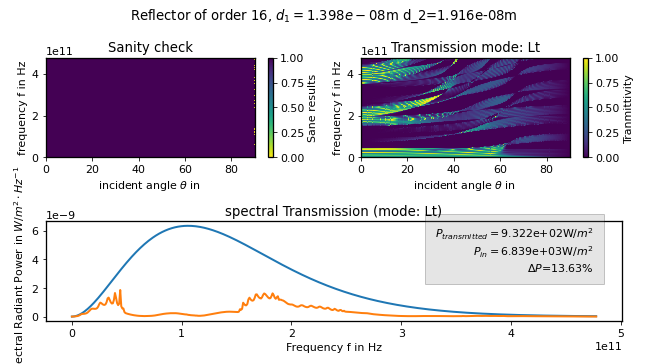
\includegraphics[width=\textwidth]{Example2/L_singlelse.png}
    \caption{Scattering of L polarised waves at a single interface calculated 
    with LSE Method}
    \label{fig:totalMultiL}
\end{figure}

\begin{figure}[h]
    \centering
    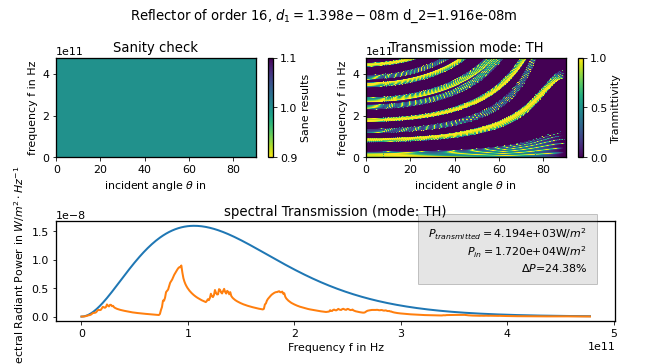
\includegraphics[width=\textwidth]{Example2/TH_singlelse.png}
    \caption{Scattering of TH polarised waves at a single interface calculated 
    with LSE Method}
    \label{fig:totalMultiTH}
\end{figure}

\begin{figure}[h]
    \centering
    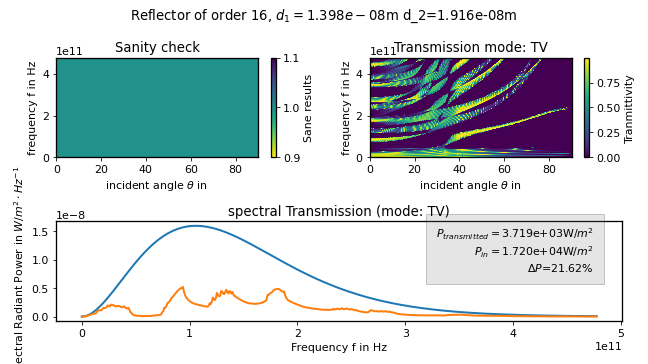
\includegraphics[width=\textwidth]{Example2/TV_singlelse.png}
    \caption{Scattering of TV polarised waves at a single interface calculated 
    with LSE Method}
    \label{fig:totalMultiTV}
\end{figure}
